\chapter{The begining}

\textit{%
This is the intro\\
multiple line
}

\section{In first place}

This is the begining of this whole thing ...

\section{a bit more}

more and more

\section{about what now ? }

Nothing :) 

but a well designed image :p 

\begin{figure}[h]
\centering
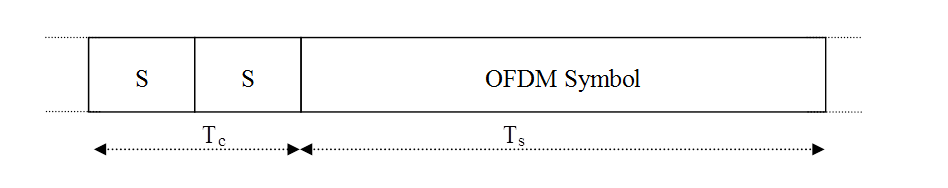
\includegraphics{src/content/img/structure_trame_tx.png}
\caption{Tux, le pingouin}
\figLabel{Tux}
\end{figure}


\begin{figure}[h]
\centering
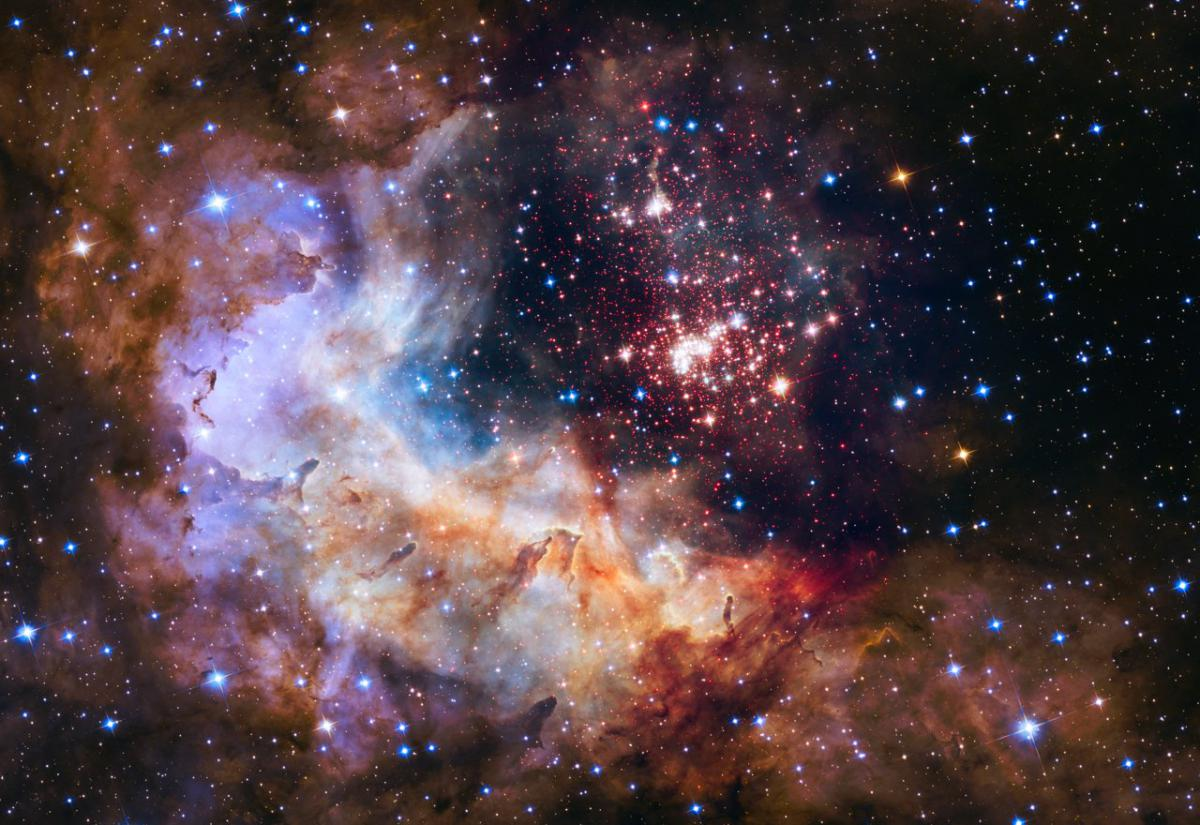
\includegraphics[width=6cm]{src/content/img/space.jpg}
\caption{Tux, le pingouin de l'espace}
\figLabel{space}
\end{figure}

Mais si l'on regarde de plus pret, Dans la \figRef{Tux}, nous lisons... ou encore \figRef{space}
\subsection{chut here detaisl}

detailed elements
